\subsubsection{Modificar Entrada de Vehículo}
En la figura \ref{fig:Diagrama de Secuencia - Modificar Entrada de Vehículo} que se muestra a continuación se muestra el flujo de las diversas actividades que corresponden a la modificación de los datos de un registro de un vehículo. En este proceso, el usuario solicita esta modificación a través del sistema y este mismo interactúa con la base de datos para su modificación. En este proceso existen algunas variantes:
\begin{itemize}
	\item \textbf{Existe de vehículo:} Se corrobora que el vehículo está registrado en la base de datos, si es así, se procede a la modificación del mismo mediante un formulario de actualización.
	\item \textbf{No existe el vehículo:} Si no existe el vehículo en la base de datos, el sistema muestra un mensaje de error al usuario.
	\item \textbf{Datos válidos:} Al modificar los datos de un vehículo, el sistema valida si esa información es correcta, es decir, si los campos han sido llenados y el formato es el correspondiente con cada uno de dichos campos.
	\item \textbf{Datos no válidos:} Los datos que se quieren sobrescribir en la base de datos son incorrectos y el sistema no permite la actualización y muestra un mensaje de error.
\end{itemize}
\begin{figure}[!h]
	\centering
	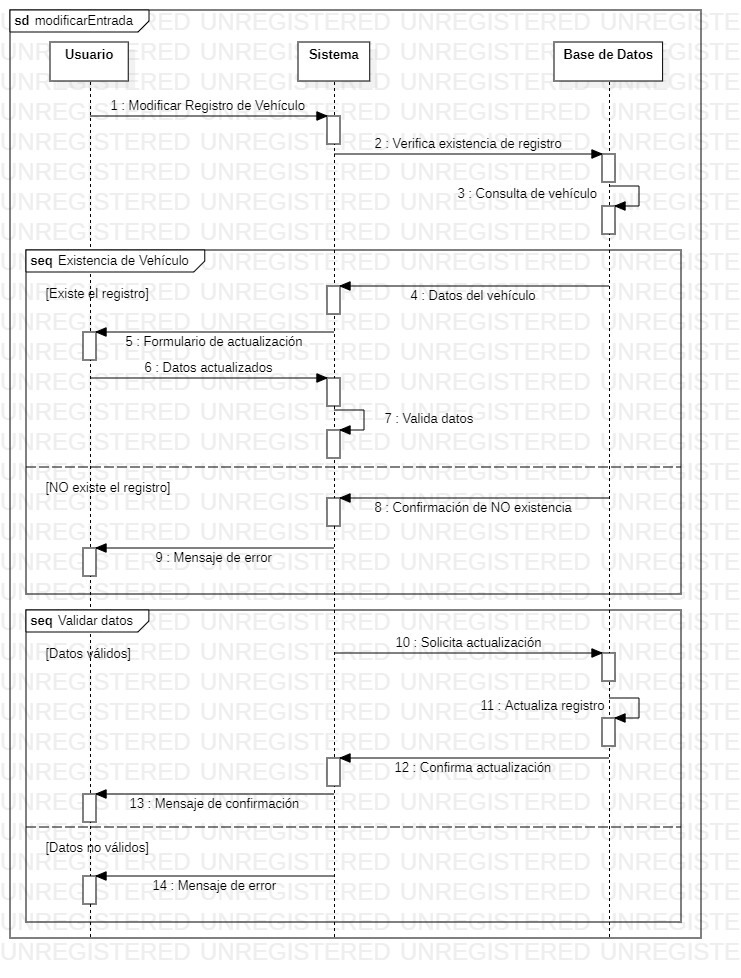
\includegraphics[width=1\textwidth]{./diseno/vprocesos/imagenes/modificarEntrada}
	\caption{Diagrama de Secuencia - Modificar Entrada de Vehículo}
	\label{fig:Diagrama de Secuencia - Modificar Entrada de Vehículo}
\end{figure}
\clearpage